\section{Results}
In this section, we first compare the number of GMRES iterations needed by
ANMG-DSA and ANMG-$P1$SA to solve a model problem. Then, both the number of
GMRES iterations and the elapsed time are compared for three methods:
\begin{itemize}
  \item Sweep preconditioning (S).
  \item DSA preconditioning (DSA).
  \item Angular multigrid (DSA variant) preconditioning (ANMG-DSA).
\end{itemize}
For every test in this section except the first one, BLD finite elements are used
and GMRES is restarted every 30 iterations. For the comparison between
ANMG-DSA and ANMG-$P1$SA GMRES is restarted every 20 iterations.
\subsection{Comparison between ANMG-DSA and ANMG-$P1$SA}
The test uses a 5$cm$ square domain, uniformly discretized using $50 \times
50$ cells. The homogeneous medium is homogeneous with a uniform isotropic source of
intensity $10 n/(cm^3 s)$ and Fokker-Planck cross sections with $\alpha=1$. 
$\Sigma_t$ is chosen to be equal to $\Sigma_{s,0}$. The quadrature is the 
Gauss-Legendre-Chebyshev triangular Galerkin quadrature. The GMRES solver is 
converged to a relative tolerance, $\(\frac{\|\textrm{residual}\|_2}{\|\textrm{right 
hand side}\|_2}\)$, of $10^{-5}$. $P1$SA is solved using BiCGSTAB with a relative 
tolerance of $10^{-7}$. DSA is solved with CG preconditioned by an algebraic 
multigrid technique \cite{pyamg,amg} with a relative tolerance of $10^{-7}$. The 
number of GMRES iterations needed to solve ANMG-DSA (multigrid preconditioner 
with $S_2$ as coarsest transport level and diffusion solve) and ANMG-$P1$SA 
(multigrid preconditioner with $S_4$ as coarsest transport level and $P1$SA solve) 
are compared (see Table \ref{table_anmg_d_p1}). The comparison is performed for 
$S_4$, $S_8$ and $S_{16}$ (for which the values of the anisotropy order $L$ are 4, 
8, 16, respectively).
\begin{table}[H]
  \begin{center}
    \caption{Comparison of the number of GMRES iterations needed in ANMG-DSA
    and ANMG-$P1$SA}
    \begin{tabular}{|c|c|c|}
      \hline
      & ANMG-DSA & ANMG-$P1$SA \\
      \hline
      $S_4$ & 21 & 19 \\
      $S_8$ & 29 & 38 \\
   $S_{16}$ & 54 & 85 \\
      \hline
    \end{tabular}
  \label{table_anmg_d_p1}
  \end{center}
\end{table}
From Table \ref{table_anmg_d_p1}, it can be seen that ANMG-DSA outperforms
ANMG-$P1$SA except for $S_4$. When the anisotropy of the problem increases,
the advantage of ANMG-DSA over ANMG-$P1$SA increases. Furthermore, we note
that the $P1$SA equations are more difficult to solve (PD but non symmetric
system) than the DSA equations (which are SPD). For these reasons, we
recommend using the ANMG-DSA variant of the angular multigrid technique.
Consequently, only the ANMG-DSA method will be employed in the later tests.
\subsection{Test Case with a Volumetric Source}
In this test, we compare ANMG-DSA to Sweep and DSA preconditioning. A uniform
isotropic source of intensity 10 $n/(cm^3 s)$ was used. $S_4$, $S_8$, $S_{16}$, and
$S_{32}$ calculations were performed. Fokker-Planck cross sections with
$\alpha=1$ are used and $\Sigma_t = \Sigma_{s,0}$ $(c=1)$. The domain is homogeneous
and its size is $5cm \times 5cm$ discretized by $50\times 50$ cells. The 
thickness of the domain varies from 50 to 2690 mean free path (the total cross 
section varies with $L$ for Fokker-Planck cross sections: $\Sigma_{t,S_4}=10cm^{-1},
\Sigma_{t,S_8}=36cm^{-1}, \Sigma_{t,S_{16}}=136cm^{-1}, 
\Sigma_{t,S_{32}}=528cm^{-1}$) but stays constant at five transport
mean free path. The relative tolerance on GMRES, which is restarted every 30
iterations, is $10^{-6}$ whereas the
relative convergence on DSA, solved by AGMG (see next Chapter), is $10^{-8}$.
The solution for $S_{32}$ calculation is given on Figure \ref{fig_s_32}
\begin{figure}[H]
  \centering
  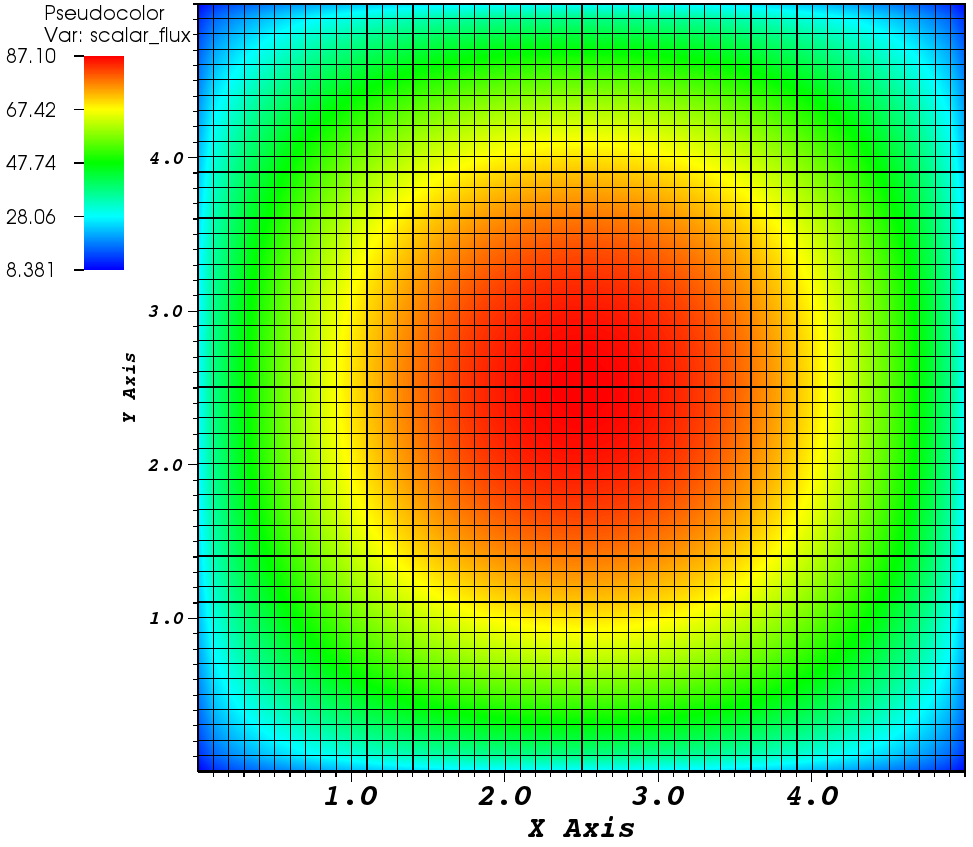
\includegraphics[width=0.6\textwidth]{Anmg/homog_anmg_crop}
  \caption{Scalar flux for the $S_{32}$ calculation on a homogeneous medium}
  \label{fig_s_32}
\end{figure}
\begin{table}[H]
  \begin{center}
    \caption{Comparison of the number of GMRES iterations needed to solve the 
      volumetric source test problem when $c=1$ using sweep preconditioning (S), DSA 
    preconditioning, and ANMG-DSA preconditioning on a homogeneous medium}
    \begin{tabular}{|c|c|c|c|c|}
      \hline
      & S & DSA & ANMG-DSA & $\frac{\textrm{ANMG-DSA}}{\textrm{DSA}}$ \\
      \hline
      $S_4$ & 85   & 42  & 27  & 0.64 \\
      $S_8$ & 409  & 102 & 50  & 0.49 \\
   $S_{16}$ & 1526 & 266 & 105 & 0.39 \\
   $S_{32}$ & 4540 & 616 & 225 & 0.36 \\
      \hline
    \end{tabular}
    \label{table_gmres_homog}
  \end{center}
\end{table}
\begin{table}[H]
  \begin{center}
    \caption{Elapsed time (s) to solve the volumetric source test problem when
      $c=1$ using sweep preconditioning (S), DSA preconditioning, and ANMG-DSA
    preconditioning on a homogeneous medium}
    \begin{tabular}{|c|c|c|c|c|}
      \hline
      & S & DSA & ANMG-DSA & $\frac{\textrm{ANMG-DSA}}{\textrm{SA}}$ \\
      \hline
      $S_4$ & 9.09322 & 6.51608 & 5.22796 & 0.80 \\
      $S_8$ & 184.949 & 52.65   & 32.7609 & 0.62 \\
   $S_{16}$ & 4275.82 & 740.193 & 355.939 & 0.48 \\
   $S_{32}$ & 138819  & 17907.9 & 7357.63 & 0.41 \\
      \hline
    \end{tabular}
    \label{table_time_homog}
  \end{center}
\end{table}
In Table \ref{table_gmres_homog}, one can note that ANMG-DSA always
requires the least number of iterations to converge. ANMG is the fastest
method (Table \ref{table_time_homog}). It took 38 hours to solve the $S_{32}$
problem with sweep preconditioning but only 2 hours when ANMG-DSA was used. As 
the anisotropy order is increased (i.e., increasing values of $L$ as a function 
of the number of directions in the Fokker-Planck cross-section representation), 
the advantage of ANMG-DSA is clear. The ratio $\(\frac{\textrm{number of GMRES 
iterations for ANMG-DSA}}{\textrm{number of GMRES iterations for DSA}}\)$ and
the ratio of elapsed times between the DSA and the ANMG-DSA
techniques decrease monotonically. We note from these results that
ANMG-DSA becomes increasingly superior to the standard DSA as the number of
directions becomes larger. The time spent performing the diffusion solve DSA is negligible
  ($\leq 1\%$ for $S_{16}$ and $S_{32}$ calculations) and is the same for DSA 
  and ANMG-DSA for a given number of CG iterations. We tried to run a problem with a $S_{64}$ GLC
  Galerkin quadrature but unfortunately we could not. The reason is that
  the function that allocates the memory for GMRES in Trilinos 
  receives the number of bytes to be allocated through an \emph{unsigned
  int} and, therefore, the maximum size of the problem per processor
  is: (number of unknowns+2) $\times$ (size of the Krylov space+1) $\times$ 8
  $\leq 4294967295$. The number of 8 is because \emph{double} are coded using
  8 bytes and 4294967295 is the largest number of representable by an
  \emph{unsigned int}. With $S_{64}$ this problem requires
  5158400496 bytes. This number is about 20\% larger than what is allowed in
  Trilinos implementation. Moreover, in the function allocating the memory, the \emph{unsigned 
  int} is cast on a \emph{int} before the allocation is done reducing the size
  of the largest problem by two. To run the $S_{64}$ problem, GMRES can be
  restarted more often but this leads to a very slow convergence.
\subsection{Test Case with a Volumetric Source with finer mesh cell sizes}
The domain is a 6$cm-$side square discretized by
  $600\times600$ cells. The quadrature used is a $S_4$ GLC Galerkin
  quadrature. There is a uniform source of intensity 10 $n/(cm^3s)$.
  Fokker-Planck cross sections are used with $\alpha=1$ and
  $\Sigma_t=\Sigma_{s,0}$ $(c=1)$. In Table
  \ref{new_gmres}, we compare the number of GMRES iterations used by Sweep
  preconditioning, DSA preconditioning, angular multigrid
  preconditioning. In Table \ref{new_time}, the time needed to solve 
  this problem is compared.
  \begin{table}[H]
    \begin{center}
      \caption{Comparison of the number of GMRES iterations needed to solve a
      problem whose infinity medium version is unstable for ANMG-DSA with SI}
      \begin{tabular}{|c|c|c|}
        \hline
         S & DSA & ANMG-DSA\\
        \hline
        101 & 47 & 29 \\
        \hline
      \end{tabular}
      \label{new_gmres}
    \end{center}
  \end{table}
  \begin{table}[H]
    \begin{center}
      \caption{Elapsed time (s) to solve a
      problem whose infinity medium version is unstable for ANMG-DSA with SI}
      \begin{tabular}{|c|c|c|}
        \hline
         S & DSA & ANMG-DSA\\
        \hline
        2767.87 & 1730.73 & 1314.07 \\
        \hline
      \end{tabular}
      \label{new_time}
    \end{center}
  \end{table}
  We note that ANMG-DSA requires fewer iterations and less time than DSA which 
  itself requires fewer iterations and less time than Sweep preconditioning.
  Using ANMG-DSA within GMRES is more efficient than DSA within GMRES,
  contrarily to what happens when SI is used. According to \cite{shawn_phd},
  if the medium is infinite, the spectral radius of the unfiltered ANMG method 
  with SI, for such a test with fine mesh cells sizes, is 2.11. Because of leakage, unfiltered ANMG with SI would probably 
  be convergent for this test but it should
  be less efficient than SI+DSA. The fact that ANMG-DSA with GMRES requires
  fewer iterations than DSA with GMRES is an indication that ANMG-DSA
with GMRES is probably stable even if there is no leakage.
\subsection{Test Case with a Heterogeneous Medium (Beam problem)}
In this test, we apply a boundary source of intensity 10 $n/(cm^2 s)$ to the
entire left side of the domain $y \in [0cm,5cm]$. The top, the bottom, 
and the right boundary conditions are vacuum. The beam intensity is only 
non-zero in the most-normal directions of the quadrature. An $S_{16}$ Galerkin 
Gauss-Legendre-Chebyshev quadrature is used. The domain
is discretized using $50 \times 50$ cells and is composed of two materials:
\begin{description}
  \item[Material 1:] for $x\in [0cm,3cm]$, Fokker-Planck cross section is used with 
    $\alpha=0.099$, $\Sigma_t = 13.6 cm^{-1}$, $c=0.99$
  \item[Material 2:] for $x\in [3cm,5cm]$, Fokker-Planck cross section is used with 
    $\alpha=9.999$, $\Sigma_t = 1360 cm^{-1}$, $c=0.99$
\end{description}
Like previously, the relative tolerance on GMRES, which is restarted every 30
iterations, is $10^{-6}$ and the relative tolerance on DSA is $10^{-8}$. 
\begin{figure}[H]
  \centering
  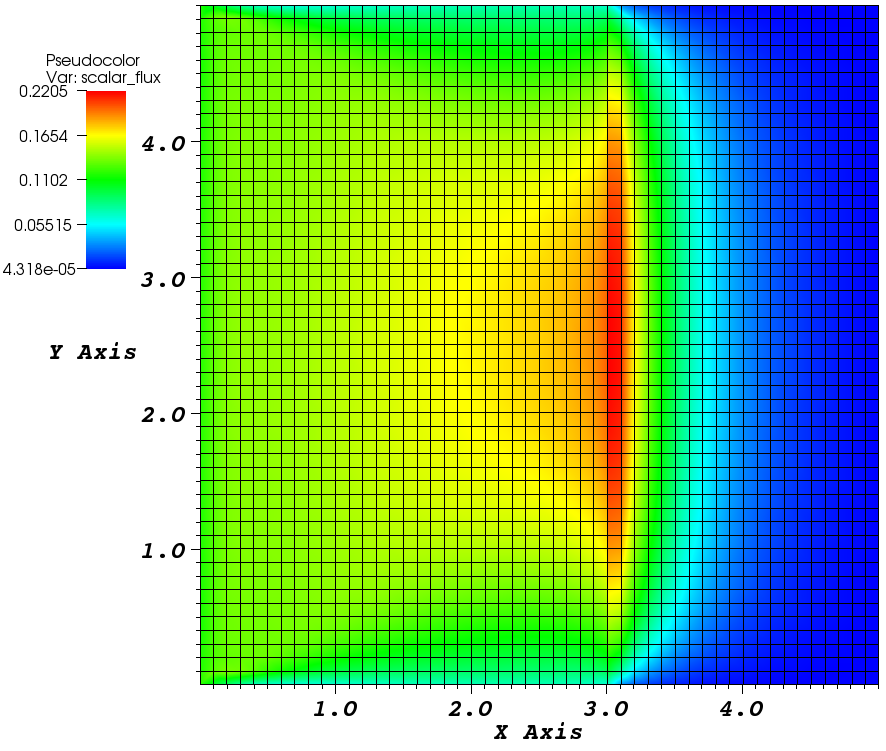
\includegraphics[width=0.6\textwidth]{Anmg/heterog_anmg_crop}
  \caption{Scalar flux for the $S_{32}$ calculation on a heterogeneous medium}
\end{figure}
The number of GMRES iterations and the elapsed 
time are given in Table \ref{table_gmres_heter} and Table \ref{table_time_heter}.
\begin{table}[H]
  \begin{center}
    \caption{GMRES iterations to solve the heterogeneous problem using sweep
    preconditioning (S), DSA preconditioning, and ANMG-DSA preconditioning on
    a heterogeneous medium}
    \begin{tabular}{|c|c|c|}
      \hline
      S & DSA & ANMG-DSA \\
      \hline
      5001 & 283 & 96 \\
      \hline
    \end{tabular}
    \label{table_gmres_heter}
  \end{center}
\end{table}
\begin{table}[H]
  \begin{center}
    \caption{Elapsed time (s) to solve the heterogeneous problem using sweep
    preconditioning (S), DSA preconditioning, and ANMG-DSA preconditioning on
    a heterogeneous medium}
    \begin{tabular}{|c|c|c|}
      \hline
      S & DSA & ANMG-DSA \\
      \hline
      13642.8 & 897.072& 394.965 \\
      \hline
    \end{tabular}
    \label{table_time_heter}
  \end{center}
\end{table}
We can see that even for a heterogeneous problem the angular multigrid is the
most effective. If we compare Table \ref{table_gmres_homog} when the 
  $S_{16}$ quadrature is used with Table \ref{table_gmres_heter}, we see that
the number of iterations needed with DSA and ANMG-DSA preconditioning are
quite similar. Sweep preconditioning, however, requires more iterations for 
the heterogeneous case because Material 2 is much thicker. We notice the same
behavior when comparing Table \ref{table_time_homog} and Table
\ref{table_time_heter} for CPU times.
